\only<2>{
\begin{textblock*}{90mm}(20mm,.3\textheight)
\begin{block}{}
Windsurfers began at the beach in 1977
\end{block}

\begin{block}{}
\includegraphic[width=1\linewidth]{graphics/}
\end{block} 

\end{textblock*}
}
\only<3>{
\begin{textblock*}{90mm}(20mm,.3\textheight)
\begin{block}{}
 Started slow but gradually as more people got into the sport a group of ``\death{regulars}" was established
\end{block}

\begin{block}{}
\includegraphic[width=1\linewidth]{graphics/}
\end{block}

\end{textblock*}
}
\only<4>{
\begin{textblock*}{90mm}(20mm,.3\textheight)
\begin{block}{}
These people spent time together and almost totally avoided interacting with other beach users who were not windsurfers
\end{block}

\begin{block}{}
\includegraphic[width=1\linewidth]{graphics/}
\end{block}

\end{textblock*}
}
\only<4>{
\begin{textblock*}{90mm}(20mm,.3\textheight)
\begin{block}{}
This produced insulated group dynamics and a ``community" bound together by a common activity
\end{block}

\begin{block}{}
\includegraphic[width=1\linewidth]{graphics/}
\end{block}

\end{textblock*}
}
\only<5>{
\begin{textblock*}{90mm}(20mm,.3\textheight)
\begin{block}{}
By  1983, stable  membership  of  about  25  to  30 (\death{Group1})
\end{block}

\begin{block}{}
\includegraphic[width=1\linewidth]{graphics/}
\end{block}

\end{textblock*}
}
\only<6>{
\begin{textblock*}{90mm}(20mm,.3\textheight)
\begin{block}{}
That same  year (1983),  the  sport  of  windsurfing  experienced  an  upsurge of  interest
\end{block}

\begin{block}{}
\includegraphic[width=1\linewidth]{graphics/}
\end{block}

\end{textblock*}
}
\only<7>{
\begin{textblock*}{90mm}(20mm,.3\textheight)
\begin{block}{}
Beginners  took  it  up  in  increasing  numbers 
\end{block}

\begin{block}{}
\includegraphic[width=1\linewidth]{graphics/}
\end{block}

\end{textblock*}
}
\only<7>{
\begin{textblock*}{90mm}(20mm,.3\textheight)
\begin{block}{}
The  established  windsurfers began to  refused  to  welcome  new  windsurfers 
\end{block}

\begin{block}{}
\includegraphic[width=1\linewidth]{graphics/}
\end{block}

\end{textblock*}
}
\only<8>{
\begin{textblock*}{90mm}(20mm,.3\textheight)
\begin{block}{}
At  first,  the  new  wave  of  beginners  were  social  isolates;  at  best,  they  were  marginal  to the  established  windsurfing  group
\end{block}

\begin{block}{}
\includegraphic[width=1\linewidth]{graphics/}
\end{block}
\end{textblock*}
}
\only<9>{
\begin{textblock*}{90mm}(20mm,.3\textheight)
\begin{block}{}
Then,  gradually,  as their  numbers  grew,  these  newcomers  began  to  drift  together  to  form  a  second  informal  group (\death{Group2})
\end{block}

\begin{block}{}
\includegraphic[width=1\linewidth]{graphics/}
\end{block}
\end{textblock*}
}
\only<10>{
\begin{textblock*}{90mm}(20mm,.3\textheight)
\begin{block}{}
Members  of  each  group  seemed,  to  some  degree,  to  limit  their  interaction  to  fellow group  members
\end{block}

\begin{block}{}
\includegraphic[width=1\linewidth]{graphics/}
\end{block}
\end{textblock*}
}
\only<10>{
\begin{textblock*}{90mm}(20mm,.3\textheight)
\begin{block}{}
Thus,  group  identities  seemed,  to  some  degree,  to  be  visible,  both  through  the 
tendency  to  limit  interaction  primarily  to  in-group  members  and  the  tendency  for 
members  of  each  group  to  locate  themselves  in  a  more  or  less compact  physical  area
\end{block}

\begin{block}{}
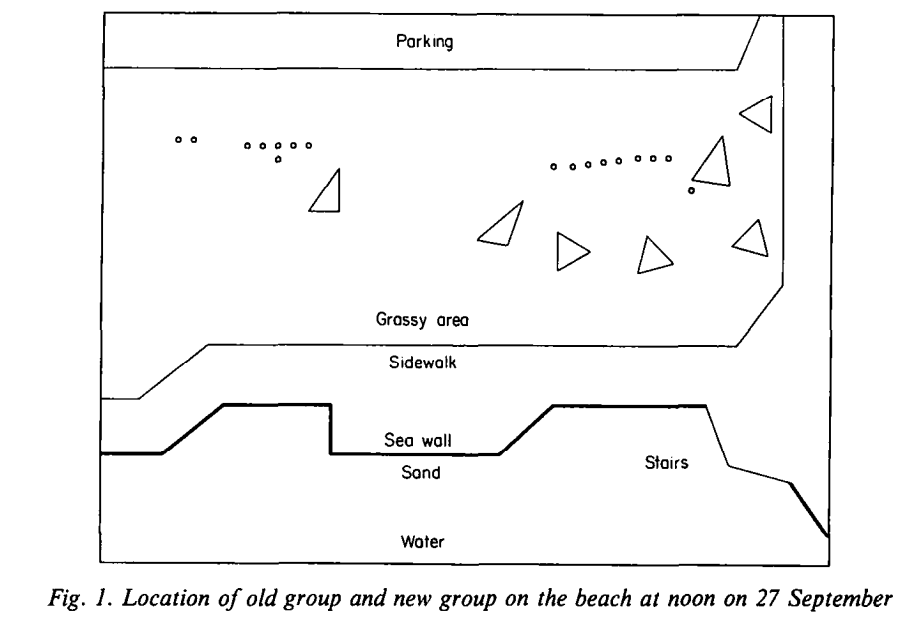
\includegraphics[width=1\linewidth]{graphics/mapLinFreeman.png}

\small
``Figure  1 shows where  people  (and  their  sails)  were  located  on  the  beach  at  noon  on  27 September  and illustrates  this [two groups]  separation" \citep{freeman88}
\end{block}

\end{textblock*}
}





